\documentclass[addpoints,11pt]{exam}

\usepackage{alltt}
\usepackage[margin=1in]{geometry}   % set up margins
\usepackage[T1]{fontenc}
\usepackage[usenames,dvipsnames]{xcolor}
\usepackage{enumerate}              % fancy enumerate
\usepackage{amsmath}                % used for \eqref{} in this document
\usepackage{amsthm}
\theoremstyle{definition}
\newtheorem{exmp}{Example}[section]
\usepackage{verbatim}               % useful for \begin{comment} and \end{comment}
\usepackage{eurosym}                % used for euro symbol
\usepackage{caption} 
\usepackage{graphicx}
\graphicspath{{Figures/}}
\usepackage{subcaption}
\usepackage{color}
\usepackage{float}
\usepackage{amssymb}
\usepackage{sgamevar}
\usepackage{sgame}
\usepackage[colorlinks=true]{hyperref}
\hypersetup{colorlinks=true, citecolor=ForestGreen, linkcolor=BlueViolet, urlcolor=Magenta}



%Solutions or nah (blank next two lines out for no solutions, unblank #3)
%\printanswers
%\newcommand{\dd}[1]{\par {\textbf{\textcolor{red}{#1}}}}
\newcommand{\dd}[1]{}  


\setlength\parindent{0pt}
\unframedsolutions
\SolutionEmphasis{\color{red}}
\CorrectChoiceEmphasis{\color{red}}
\renewcommand{\choicelabel}{(\alph{choice})}
\newcommand{\blank}[0]{\underline{\hspace{3cm}}}
\pointformat{\bfseries[\thepoints]}
\pointpoints{pt}{pts}
\pointsinrightmargin


\begin{document}


	\title{\textbf{Problem Set 5 \dd{Answers and Selected Solutions}} \\ \vspace{2 mm} {\large Principles of Economics}}
	\author{David A. D\'iaz}
	\date{}
	\maketitle

\subsection*{Economic Growth}

\begin{questions}
	
	\question The Peapod Restaurant uses all of the following to produce vegetarian meals. Which of
	them is an example of physical capital?
	
	\begin{choices}
		\choice The owner's knowledge of how to prepare vegetarian entrees.
		\choice The money in the owner's account at the bank she borrowed money from.
		\CorrectChoice The tables and chairs in the restaurant.
		\choice The land the restaurant was built on.
	\end{choices}
	
	\begin{solution}
		Physical capital is the stock of equipment used to produce goods and services.
	\end{solution}
	
	\question Institutions are thought to be the \blank causes of economic growth.
	
	\begin{choices}
		\choice proximate 
		\choice immediate 
		\CorrectChoice ultimate
		\choice direct
	\end{choices}
	
	\begin{solution}
		See class notes.
	\end{solution}
	
	
	\question Because capital is subject to diminishing returns, higher saving and investment does not lead to higher
	
	\begin{choices}
		\choice growth in the short run.
		\CorrectChoice growth in the long run.
		\choice income in the short run.
		\choice income in the long run.
	\end{choices}
	
	\begin{solution}
		Growth in the long run is limited due to diminshing returns to capital. Sustained growth is the result of innovation and improvements in technology.
	\end{solution}
	
	
	\question Which of the following would be considered an increase in human capital?
	
	\begin{choices}
		\CorrectChoice An increase in the training of heart disease researchers.
		\choice An increase in the use of heart disease centers.
		\choice The discovery of a cure for broken hearts.
		\choice An increase in the number of heart disease researchers.
	\end{choices}
	
	\begin{solution}
		Human capital is the knowledge and skills that workers acquire through education, training, and experience.
	\end{solution}
	
	\question Which of the following is NOT a determinant of a country's long-run productivity?
	
	\begin{choices}
		\choice Natural resources
		\choice Human capital
		\CorrectChoice Money supply
		\choice Physical capital
	\end{choices}
	
	\begin{solution}
		See class notes.
	\end{solution}
	
	
	\question Which of the following is NOT a kind of institution encouraging investment and the efficient organization of the factors of production?
	
	\begin{choices}
		\choice Dependable legal system
		\choice Political stability
		\choice Honest government
		\CorrectChoice Social safety nets
	\end{choices}
	
	\begin{solution}
		See class notes.
	\end{solution}
	
	\question If a country's real GDP per capita was \$40,000 in 1980 and grew to \$80,000 in 2010, then the country's annual growth rate during this period would have been approximately 
	
	\begin{choices}
		\CorrectChoice 2.3\%.
		\choice 50\%.
		\choice 3\%.
		\choice 100\%.
	\end{choices}
	
	\begin{solution}
		Country doubled it real GDP per capital in 30 years. Rule of 70: Doubling time $\approx$ 70/g $\Rightarrow$ 30 = 70/g $\Rightarrow$ g = 70/30 = 2.33\%.
	\end{solution}
	
	\question Suppose the real GDP in Slovenia in 1950 was \$50,000. If by 1977, the real GDP was \$200,000, what was the approximate annual growth rate in the country from 1950 to 1977?
	
	\begin{choices}
		\choice 2.6\%
		\choice 300\%
		\choice 4.0\%
		\CorrectChoice 5.2\%
	\end{choices}
	
	\begin{solution}
		Similar calculation as the last question, but GDP doubled twice (quadrupled) in 27 years. g = $2\times(70/27) = 5.2\%$.
	\end{solution}
	
\question The opportunity cost of growth is 

\begin{choices}
	\choice a reduction in current investment.
	\choice a reduction in current savings.
	\CorrectChoice a reduction in current consumption
	\choice a reduction in taxes.
\end{choices}

\question If a production function exhibits constant returns to scale, 

\begin{choices}
	\choice doubling all of the inputs has absolutely no impact on output because output is constant.
	\CorrectChoice doubling all of the inputs doubles output.
	\choice doubling all of the inputs more than doubles output due to the catch-up effect.
	\choice doubling all of the inputs less than doubles output due to diminishing returns.
\end{choices}

\question Our standard of living is most closely related to 

\begin{choices}
	\choice how hard we work.
	\choice our supply of capital.
	\choice our supply of natural resources.
	\CorrectChoice our productivity.
\end{choices}

\newpage

\question Which of the following statements is true?

\begin{choices}
	\choice Countries may have a different level of GDP per person, but they all grow at the same rate.
	\choice Countries may have a different growth rate, but they all have the same level of GDP per person.
	\choice Countries all have the same growth rate and level of output because any country can obtain the same factors of production.
	\CorrectChoice Countries have great variance in both the level and growth rate of GDP per person; thus, poor countries can become relatively rich over time.
\end{choices}

\question Which of the following describes an increase in technological knowledge?

\begin{choices}
	\CorrectChoice A farmer discovers that it is better to plant in the spring rather than in the fall.
	\choice A farmer buys another tractor.
	\choice A farmer hires another day laborer.
	\choice A farmer sends his child to agricultural college and the child returns to work on the farm.
\end{choices}

\question Which of the following government policies is \textit{least} likely to increase growth?

\begin{choices}
	\choice An increase in expenditures on public education
	\CorrectChoice Increased restrictions on foreign imports.
	\choice Reduce restrictions on foreign capital investment.
	\choice Eliminate corruption in the legislative branch.
\end{choices}

\question To increase growth, governments should do all of the following except

\begin{choices}
	\choice promote free trade.
	\choice encourage saving and investment.
	\choice encourage foreigners to invest in their country.
	\choice encourage research and development.
	\CorrectChoice nationalize major industries.
\end{choices}
	
\end{questions}

\subsection*{The Solow Model}

\begin{questions}
	
	
	\question Suppose the production function in the United States was $y = \sqrt{k}$ before the Information Technology revolution took place. Assume the depreciation rate is 5\% and the country invests 30\% of its output. After the revolution, productivity increased by 50\%. Suppose that at the time of the change, $k_0 = 36$. This implies that the economy moved from \blank economic growth to \blank growth. 
	
	\begin{choices}
		\choice positive; positive
		\choice positive; zero
		\CorrectChoice zero; positive
		\choice negative; positive
	\end{choices}
	
	\begin{solution}
		Before the IT revolution: $y = \sqrt{k} \Rightarrow A = 1$ \& $i = .3\sqrt{k}$. $d=.05k$. $k_0 = 36 \Rightarrow i = .3(6) = 1.8$ \& $d= .05(36) = 1.8$. Since $i=d$ there will be zero economic growth (country is at its steady state). \\
		After IT revolution: $A = 1(1.5) =1.5 \Rightarrow y=1.5\sqrt{k} \Rightarrow i = .3(1.5\sqrt{k}) = .45(6) = 2.7.$ Depreciation is still 1.8. Since $i>d$, the country will experience positive economic growth.
	\end{solution} 
	
\newpage
	
	\question Suppose a country is currently at its steady state. If the country's population growth rate permanently increases from 2\% to 4\%, which of the following must be true?
	
	
	\begin{enumerate}[i.]
		\item The new steady state consumption level will be greater than the old steady state consumption level.
		\item Investment will immediately decrease, and the new steady state investment level will be less than the old steady state investment level.
		\item The new steady state level of capital will be less than the old steady state level of capital, and the new steady state level of output will be less than the old steady state level of output.
	\end{enumerate}
	
	\begin{choices}
		\choice i and ii
		\choice ii and iii
		\choice i only
		\CorrectChoice iii only
		\choice i, ii, and iii
	\end{choices}
	
	\question If output per worker in an economy is 20, and the investment function is given by $i = .25y$, then
	
	\begin{choices}
		\choice 20 units of output are being invested.
		\choice 15 units of output are being invested.
		\choice 20 units of output are being consumed.
		\CorrectChoice 15 units of output are being consumed.
	\end{choices}
	
	
	\begin{solution}
		$i=.25(20) = 5$. $c = y - i = 20 - 5 = 15$.
	\end{solution}
	
	\question Country $X$ and country $Y$ both have the same production function, $f(k)=1.5\sqrt{k}$. Moreover, the current level of capital per worker in each country is $k_0 = 400$. In country $X$, output per worker is growing, while in country $Y$ it is falling. According to the Solow Model, \textit{ceteris paribus}, which of the following could account for this difference?
	
	\begin{choices}
		\CorrectChoice The savings rate in country $X$ is greater than that in country $Y$.
		\choice The population growth rate in country $X$ is greater than that in country $Y$.
		\choice Capital depreciates faster in country $X$ than in country $Y$.
		\choice Any of the above could account for this difference.
		\choice None of the above could account for this difference.
	\end{choices}
	
	\begin{solution}
		Country $X$ must be below its steady state since output is growing, while country $Y$ must be above its steady state. Thus country $X$ must have a higher savings rate. Each of the other options would imply that country $X$ has a lower steady state level of output than country $Y$.
	\end{solution}
	
	\question Suppose a country is currently at its steady state. If the country decides to permanently decrease its savings rate, which of the following must be true?
	
	
	\begin{enumerate}[i.]
		\item Consumption will immediately increase, and the new steady state consumption level will be greater than the old steady state consumption level.
		\item Investment will immediately decrease, and the new steady state investment level will be less than the old steady state investment level.
		\item The new steady state level of capital will be less than the old steady state level of capital, and the new steady state level of output will be less than the old steady state level of output.
	\end{enumerate}
	
\newpage
	
	\begin{choices}
		\choice i and ii
		\choice i and iii
		\CorrectChoice ii and iii
		\choice i, ii, and iii
	\end{choices}
	
	\begin{solution}
		See class notes. Consumption will immediately decrease, but may be higher or lower at the new steady state depending on the savings rate. Thus (i) is not necessarily true.
	\end{solution}

	
	\question Figure \ref{MC22} shows the production function of a small country, as well as its investment and depreciation functions. Assume there is no population growth.
	
	
	\begin{figure}[H]
		\centering
		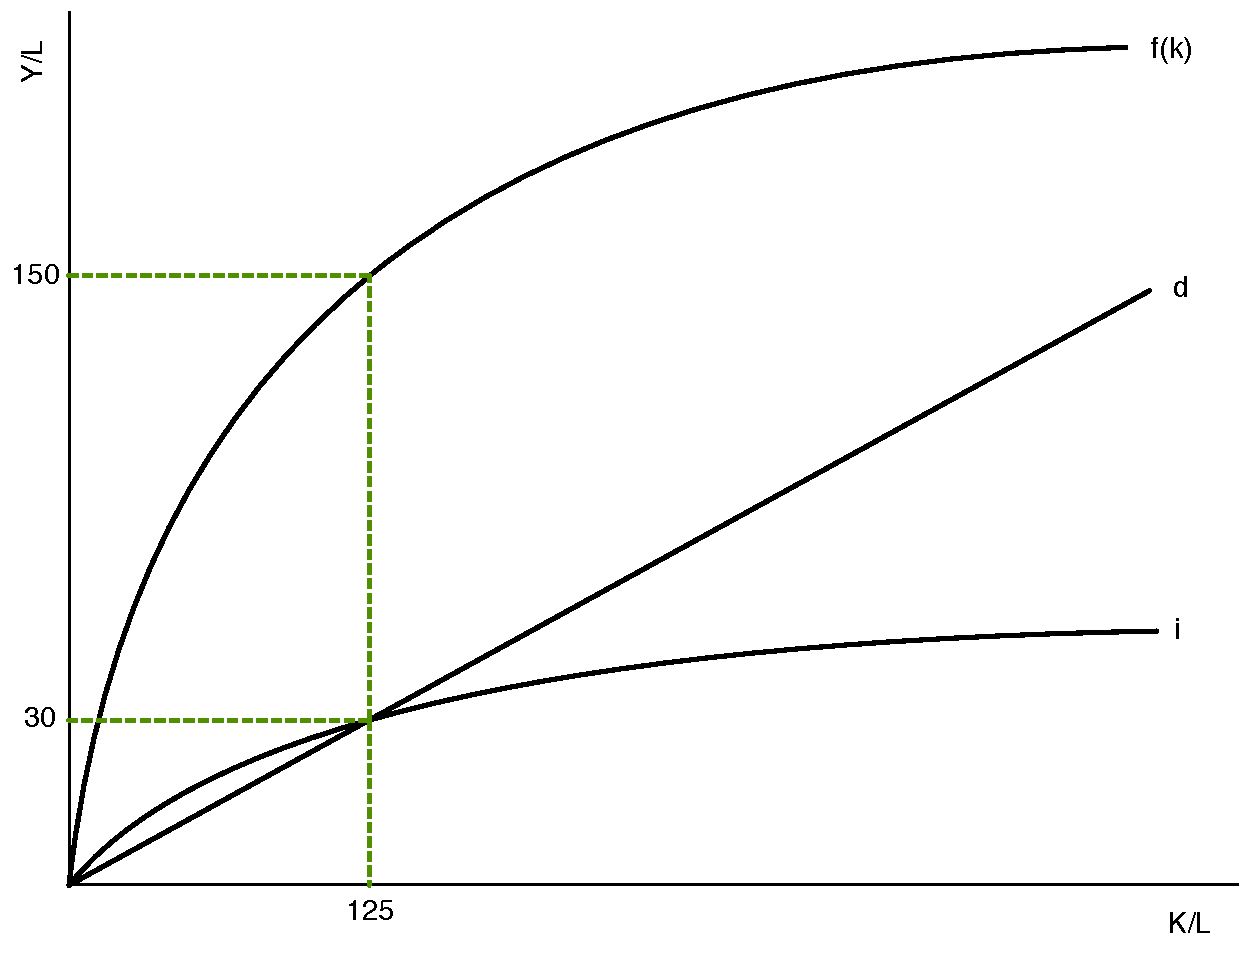
\includegraphics[scale=.4]{Final_MC22.pdf}
		\caption{Production, Investment, and Depreciation}
		\label{MC22}
	\end{figure}
	
	The percent of output per worker that is invested every period is \blank and the rate of capital depreciation is \blank.
	
	\begin{choices}
		\choice 20\%; 20\%
		\choice 24\%; 20\%
		\choice 24\%; 24\%
		\CorrectChoice 20\%; 24\%
	\end{choices}
	

	
	
	\uplevel{Use the following to answer questions \ref{blah1}-\ref{blah2}. Each worker in an economy has a capital stock of 900 units and a production function given by $y = \sqrt{k}$. This year it consumed 10 units of output and 10\% of its capital stock depreciates every year.} 
	
	
	
	\question \label{blah1} \textit{Ceteris paribus}, what will the growth rate in this country be over the next year?
	
	\begin{choices}
		\CorrectChoice $-3.96\%$
		\choice 10\%
		\choice 2.4\%
		\choice $-4.13\%$
	\end{choices}
	
	\begin{solution}
		$y = \sqrt{900} = 30 \Rightarrow i = 30 - 10 = 20$. $d = 900(.10) = 90$. Capital next year = capital today + investment - depreciation = 900 + 20 - 90 = 830 $\Rightarrow$ output next year = $\sqrt{830}$ = 28.81 $\Rightarrow \hat{y} = (28.81 - 30)/30 = -3.96\%$.
	\end{solution}
	
\newpage
	
	\question \label{blah2} If instead, the country had 20\% of its capital stock depreciate every year, what will its level of capital \ per worker be next year?
	
	\begin{choices}
		\choice 920 units
		\choice 720 units
		\choice 900 units
		\CorrectChoice 740 units
	\end{choices}
	
	\begin{solution}
		$d = .20(900) = 180$. $k_{1} = 900 + 20 - 180 = 740$.
	\end{solution}
	
	
	
	\question Figure \ref{MC30} shows the production, investment, and depreciation functions of Iceland.
	
	\begin{figure}[H]
		\centering
		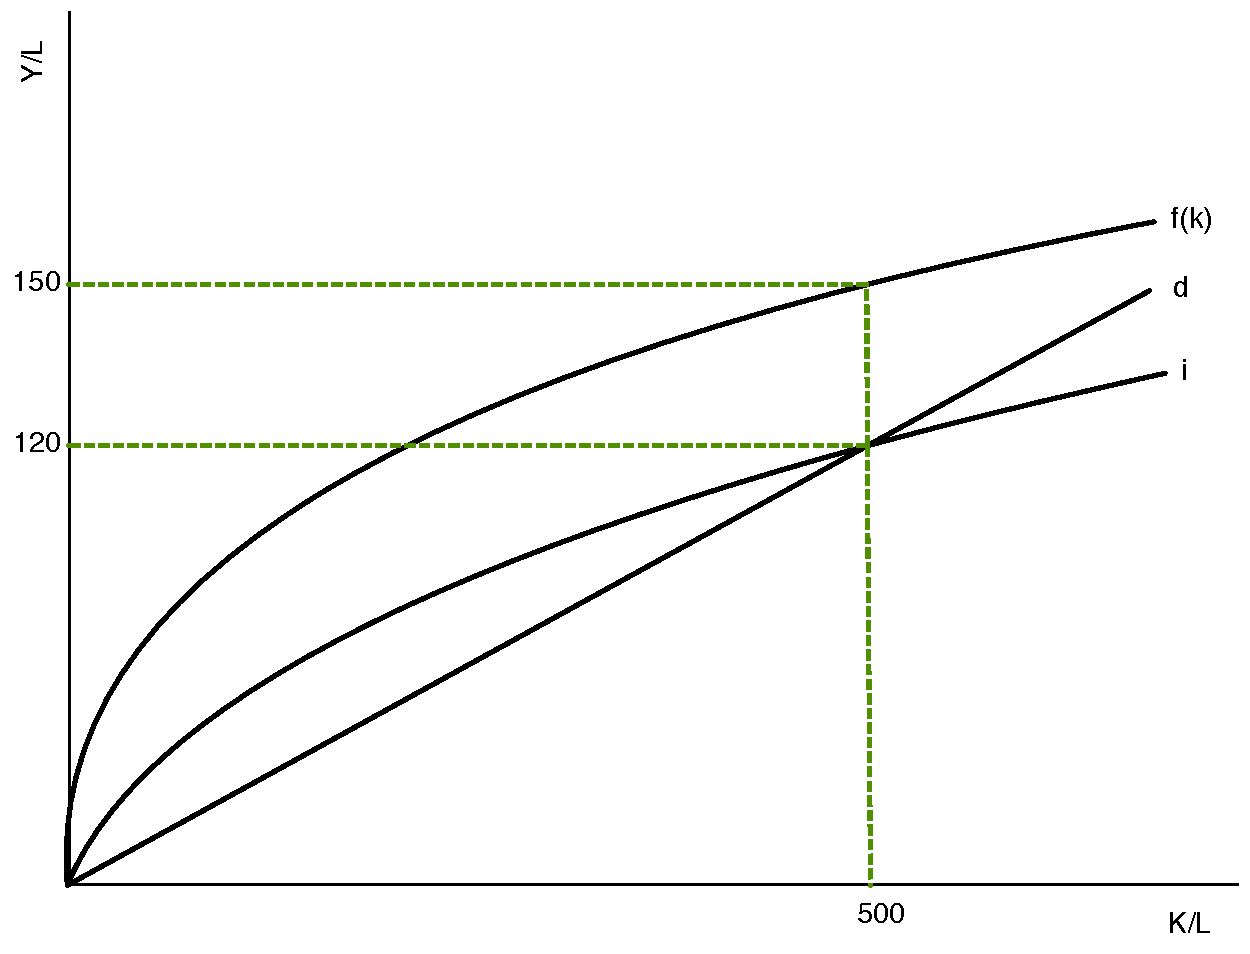
\includegraphics[scale=.40]{Exam2_MC30.pdf}
		\caption{Production in Iceland}
		\label{MC30}
	\end{figure}
	
	The amount of capital per worker that depreciates each period in the steady state is \\ \blank and the percent of output per worker that is consumed in the steady state is \blank.
	
	\begin{choices}
		\choice 500; 80\%
		\CorrectChoice 120; 20\%
		\choice 500; 20\%
		\choice 120; 80\%
	\end{choices}
	
	\begin{solution}
		Steady state where $i=d$. Steady state level of capital is 500, investment is 120, output is 150, and consumption is $150-120=30$. $d^* = i^* = 120$. Percent of output consumed = 30/150 = 20\%.
	\end{solution}
	
\question An economy has the production function $y = \sqrt{k}$. If the savings rate is 30\%, the depreciation rate is 3\%, and population growth is zero, then the steady state level of consumption per worker is

\begin{choices}
	\choice 10.
	\choice 3.
	\CorrectChoice 7.
	\choice 5.
\end{choices}

\newpage

\question Suppose a country has the production function $y=5\sqrt{k}$. Capital depreciates at rate $\delta = 4\%$. Moreover, the labor force in the country is very elderly, and as a result the country's workforce \underline{decreases} by 2\% every period. Use this information and Table \ref{solow} to answer the questions that follow.

\begin{table}[H]
	\centering
	\caption{Solow Growth}
	\label{solow}
	\begin{tabular}{c|c|c|c|c|c}        
		
		$t$ & $k_t$ & $y_t$ & $d_t$ & $i_t$ & $\hat{y}_t$ \\
		\hline
		0 & \dd{1,600} & \dd{200}  & 32 & 32 & --- \\
		1 & \dd{1,600} & \dd{200}  & \dd{32}  & \dd{32}  & \dd{0\%}  \\
		$\cdot$ & &&&&\\
		$\cdot$ &&&&& \\
		$\cdot$ &&&&& \\
		5 & \dd{1,600} & \dd{200}  & \dd{32}  & \dd{32}  & \dd{0\%} \\
		6 &  \dd{1,600} & \dd{200}  & \dd{32}  & \dd{32}  &  $x$ \dd{= 0\%} \\
		7 & \dd{1,600} & \dd{200}  & \dd{32}  & \dd{40}  &   \\
		8 & \dd{1,608} & \dd{200.499}  &   &  & $z$ \dd{= .2495\%} \\
	\end{tabular}
\end{table}

\begin{parts}
	\part If the country is currently in period $t=0$, do you expect capital to accumulate, decumulate, or neither in the next period? Explain why.
	
	\begin{solution}
		Neither. Since $i = d$, the country is at its steady state in period 0 and so capital will not change in the next period.
	\end{solution}
	
	\part What is the level of capital and output per worker in this period ($t=0$)? 
	
	\begin{solution} 
		$d_t = (n + \delta)k_t = ((-.02) + .04)k_t = .02k_t$. $d_{0} = 32 \Rightarrow k_{0} = 32/.02 = 1,600$. $y_{0} = 5\sqrt{1,600} = 200$.
	\end{solution}
	
	\part What is the savings \underline{rate} in this country? 
	
	\begin{solution}
		$i_t = sy_t = s(200)$. $i_{0} = 32 \Rightarrow s = 32/200 = 16\%$.
	\end{solution}
	
	\part Assuming everything remains the same, what is the growth rate of output per worker in period $t=6$ (i.e., what is $x$)? 
	
	\begin{solution}
		Since the country is at its steady state, the growth rate of output per worker will be 0\% in every period unless $A$, $s$, $n$, or $\delta$ change.
	\end{solution}
	
	\part At the beginning of period $t=7$, the country changes its saving rate to 20\%. What is the growth rate of output per worker in period $t=8$ (i.e., what is $z$)? 
	
	\begin{solution}
		Since the country was at its steady state at the start of period 7, $k_{7}=1,600$ and $y_{7} = 200$. Depreciation for the period remains $d_{7}=32$, but now $i_{7} = .20(200) = 40$ since $s=20\%$. Capital at the start of period 308: $k_{8} = k_{7} + i_{7} - d_{7} = 1,600 + 40 - 32 = 1,608$. $y_{8} = 5\sqrt{1,608} = 200.499$. Growth rate of output: $\widehat{y}_{8} = (200.499 - 200)/200 = .2495\%$.
	\end{solution}
	
	\part Draw the effect of this change in the savings rate on a well-labeled graph. You do not need to write the specific numbers down, but clearly show the steady state levels of capital, output, investment, and consumption per worker before and after the change.
	
	\begin{solution}
		See class notes. The graph should depict an increase in the savings rate, which shifts the investment function up. $k^*, i^*,$ and $y^*$ all increase. The effect on $c^*$ is ambiguous.
	\end{solution}
\end{parts}


	
	\question A country has the production function $F(K,L) = A K^\beta L^{1-\beta}$, where $0<\beta<1$, $K$ represents the country's capital stock, and $L$ represents its labor force. 
	\begin{parts}
		\part Show that doubling both inputs will double the output the country can produce (i.e., $F(2K,2L) = 2F(K,L))$. What is this property called?\footnote{\textbf{Hint:} A couple of properties of exponents are that $x^a\cdot
			x^{1-a} = x^{(a+1-a)}$ and $(xy)^a = x^a\cdot y^a$.} 
		
		\begin{solution}
			$F(2K,2L) = A(2K)^\beta(2L)^{1-\beta} = A(2)^\beta(2)^{1-\beta}K^\beta L^{1-\beta} = 2^{\beta + 1 - \beta} AK^\beta L^{1-\beta} = 2(AK^\beta L^{1-\beta}) = 2F(K,L)$. This production function exhibits constant returns to scale.
		\end{solution}
		
		\part Define $k = K/L$ as the capital-labor ratio and write output per worker as $f(k) = Ak^\beta$. Suppose $A = 4$ and $\beta = 1/2$. What is the marginal product of capital per worker for the first unit of capital? The second? Third? What property does this show? 
		\begin{solution}
			$Y/L = (1/L)F(K,L) = F(K/L, L/L) = Ak^\beta \equiv f(k)$. Plugging in $A=4$ and $\beta = 1/2$, $f(k) = 4\sqrt{k}$. \\
			$f(0) = 4\sqrt{0} = 0$. \\
			$f(1) = 4\sqrt{1} = 4$. $MP_k = 4-0=4$. \\
			$f(2) = 4\sqrt{2} = 5.66$. $MP_k = 5.66-4 = 1.66$.\\
			$f(3) = 4\sqrt{3} = 6.93$. $MP_k = 6.93-5.66 = 1.27$. \\
			This production function exhibits diminishing marginal returns to capital.
		\end{solution}
		
		\part The capital stock in this country depreciates at rate $\delta=3\%$, output is invested at rate $s=15\%$, and the labor force grows at rate $n=2\%$. It currently has a capital stock per worker of $k_0 = 100$. How much, if any, capital per worker do you expect the country to accumulate (or decumulate) once it reaches its steady state?
		
		\begin{solution}
			$i = sy = .15(4\sqrt{k}) = .6\sqrt{k}$. $d=(n+\delta)k = (.02+.03)k = .05k$. SS: $.6\sqrt{k} = .05k \Rightarrow (.6)^2(\sqrt{k})^2 = (.05)^2k^2 \Rightarrow .36k = .0025k^2 \Rightarrow k^* = (.36/.0025) = 144$. Since capital is currently 100, we expect 44 units of capital to accumulate.
		\end{solution}
		
		\part What is the steady state level of output, investment, and consumption in this country? 
		
		\begin{solution}
			$y* = f(k^*) = 4\sqrt{144} = 48$. \\
			$i^* =sy^* = .15(48) = 7.2$ \\
			$c^* = (1-s)y^* = y^* - i^* = 40.8$.
		\end{solution}
	\end{parts}
	
\end{questions}


\subsection*{Savings, Investment, and the Financial System}

\begin{questions}
	

\question A closed economy has income of \$1,000, government spending of \$200, taxes of \$150, and investment of \$250. What is private saving?

\begin{choices}
	\choice \$100
	\choice \$200
	\CorrectChoice \$300
	\choice \$400
\end{choices}

\begin{solution}
	National saving = National investment. $Y - C - G = I$ $\Rightarrow 1000 - C - 200 = 250 \Rightarrow C = \$550$. Private saving = $Y - T - C = 1000 - 150 - 550 = \$300.$
\end{solution}

\question Acme, LLC is considering purchasing a new factory. If the interest rate falls, then the present value of the returns from the factory will \blank, and the company will be \\ \blank likely to build the factory.

\begin{choices}
	\choice increase; less
	\choice decrease; more
	\CorrectChoice increase; more
	\choice decrease; less
\end{choices}


\begin{solution}
	If the interest rate falls, then the cost of borrowing will decrease and so the present value of the returns increases. This will make the company more likely to build the factory.
\end{solution}


\question If the business community becomes more optimistic about the profitability of capital, the \blank for loanable funds would shift, driving the equilibrium interest rate \\  \blank.

\begin{choices}
	\choice supply; up
	\choice supply; down
	\CorrectChoice demand; up
	\choice demand; down
\end{choices}

\begin{solution}
	Demand for loanable funds will increase, which will increase the equilibrium interest rate and quantity of loanable funds.
\end{solution}

	\question Savings is 
	
	
	
	\begin{choices}
		\choice the purchase of new capital goods.
		\choice the purchase of new consumption goods.
		\choice income that is not spent on capital goods.
		\CorrectChoice income that is not spent on consumption goods. 
	\end{choices}	
	

\question What effect will an investment tax credit have on interest rates and the quantity of savings?

\begin{choices}
	\choice Both interest rates and the quantity of savings will decrease.
	\choice Interest rates will increase, and the quantity of savings will decrease.
	\CorrectChoice Both interest rates and the quantity of saving will increase.
	\choice Interest rates will decrease, and the quantity of savings will increase.
\end{choices}

\begin{solution}
	An investment tax credit will increase the demand for loanable funds. This will increase both the equilibrium interest rate and quantity of loanable funds.
\end{solution}

\newpage

\question Which of the following graphs of the loanable funds market correctly shows the effect of the imposition of a consumption tax?

\begin{figure}[H]
	\begin{subfigure}[b]{0.5\textwidth}
		\centering
	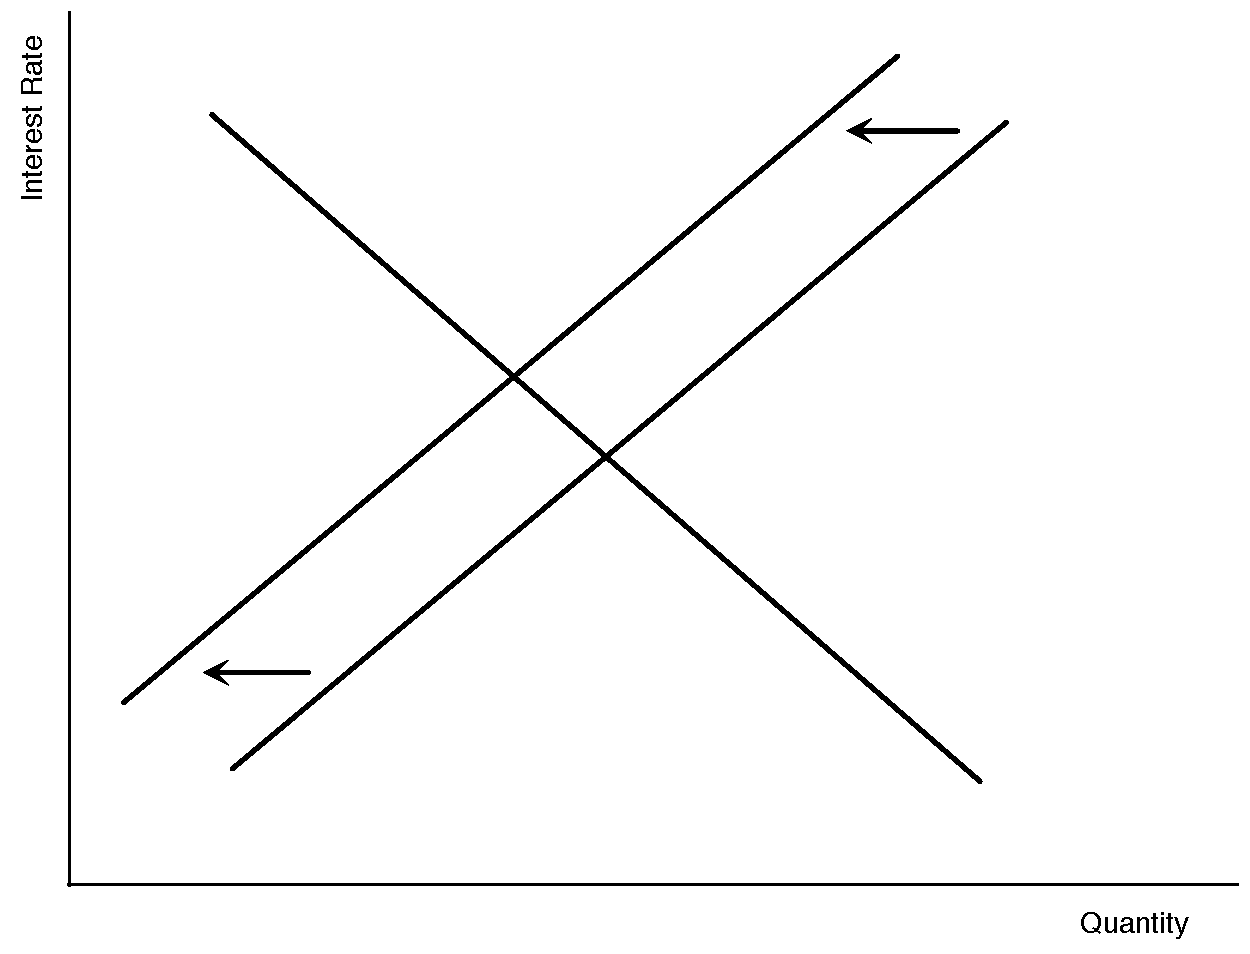
\includegraphics[scale=.35]{loans1.pdf}
		\caption{}
	\end{subfigure}
	\begin{subfigure}[b]{0.5\textwidth}
		\centering
	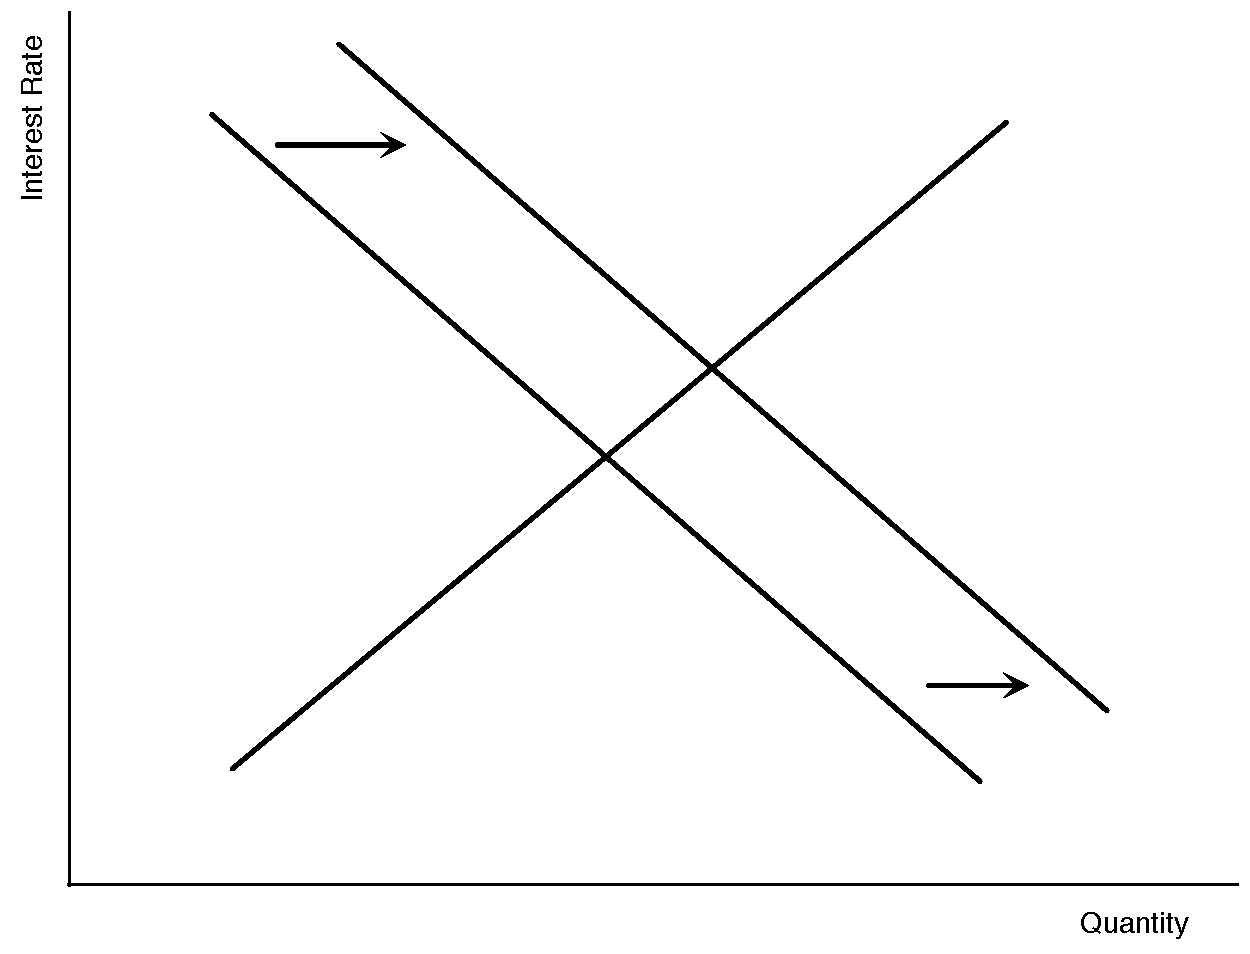
\includegraphics[scale=.35]{loans2.pdf}
		\caption{}
	\end{subfigure}
		%        
		
	\begin{subfigure}[b]{0.5\textwidth}
		\centering
		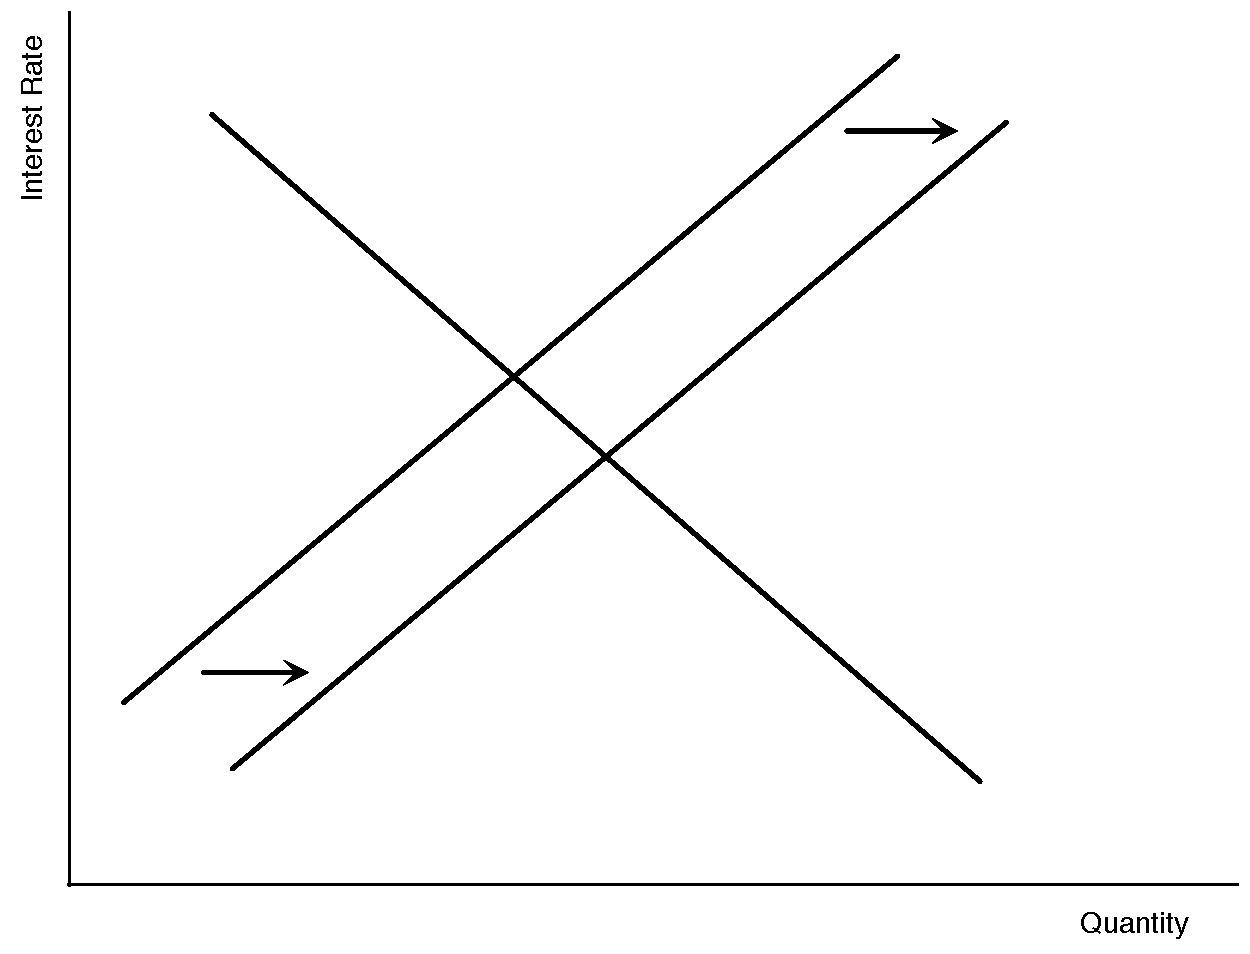
\includegraphics[scale=.35]{loans3.pdf}
		\caption{}
	\end{subfigure}
	\begin{subfigure}[b]{0.5\textwidth}
		\centering
		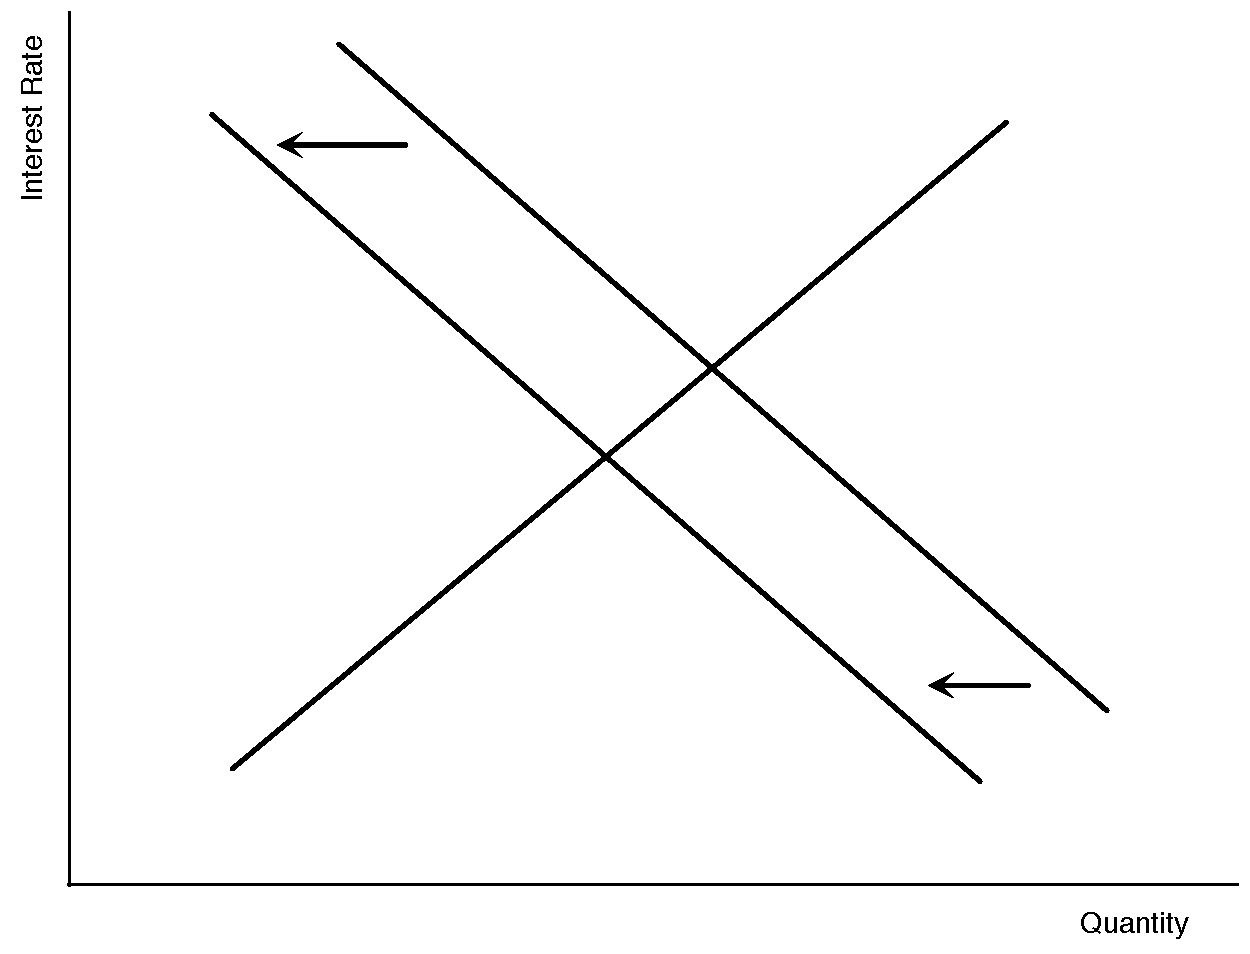
\includegraphics[scale=.35]{loans4.pdf}
		\caption{}
	\end{subfigure}
\end{figure}

\begin{solution}
	A tax on consumption provides an incentive for people to save more (since we assume you can either spend your income on savings or consumption) and so the supply of loanable funds will increase. Option (c) shows this shift.
\end{solution}

\question Always On Time Airlines is considering purchasing a new jet. The company would be \textit{less} likely to purchase a new jet if either

\begin{choices}
	\choice the price of a new jet decreased or the interest rate decreased.
	\choice the price of a new jet increased or the interest rate decreased.
	\choice the price of a new jet decreased or the interest rate increased.
	\CorrectChoice the price of a new jet increased or the interest rate increased.
\end{choices}

\begin{solution}
	The cost of borrowing increases if the price of the jet increases or interest rates increase.
\end{solution}


	
	\question Suppose you currently hold a bond that promises to pay \$100 in a year, \$100 in two years, and \$1,100 in three years. If you wish to sell the bond today in order to buy a new bicycle, which of the following market interest rates would allow you to sell the bond for the highest price?
	
	\begin{choices}
		\choice 7\%
		\choice 10\%
		\CorrectChoice 5\%
		\choice 8\%
	\end{choices}
	
\begin{solution}
	The price of a bond is inversely related to market interest rates.
\end{solution}

\question Assuming the supply of loanable funds is made up of national savings, which of the following would be the most likely to cause an increase in the demand for loanable funds?

\begin{choices}
	\choice A decrease in the interest rate.
	\choice An increase in savings.
	\choice A decrease in consumption.
	\choice An increase in government borrowing.
	\CorrectChoice None of the above.
\end{choices}

	\question Figure \ref{MC27} shows the market for loanable funds. 
	
	
	\begin{figure}[H]
		\centering
		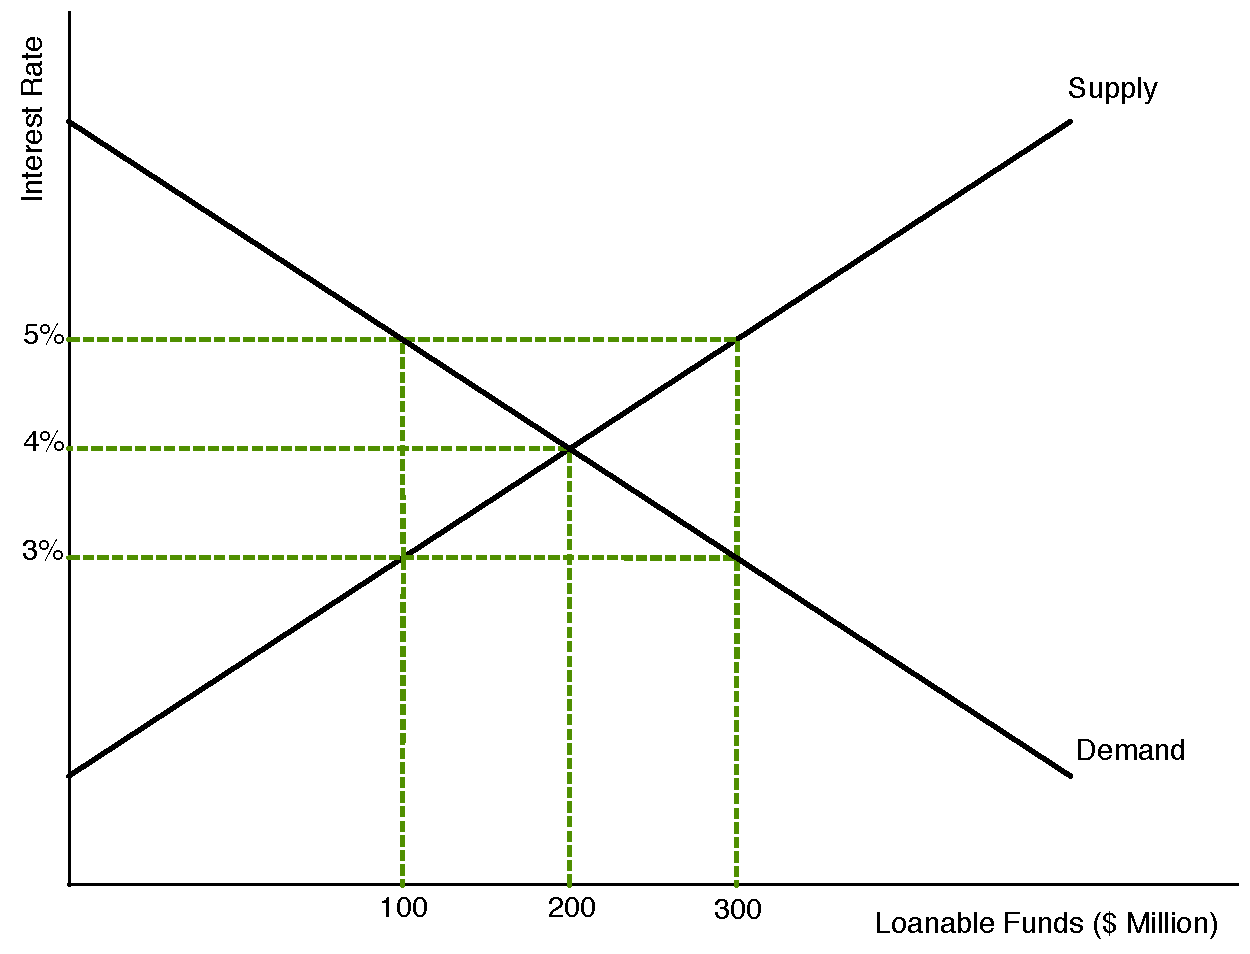
\includegraphics[scale=.4]{Exam2_MC27.pdf}
		\caption{Market for Loanable Funds}
		\label{MC27}
	\end{figure}
	
	If the interest rate in the market is 3\%, then 
	
	\begin{choices}
		\choice investment exceeds savings by \$300 million.
		\choice investment exceeds savings by \$200 million.
		\choice borrowing demands exceed savings by \$300 million.
		\CorrectChoice borrowing demands exceed savings by \$200 million.
	\end{choices}

\begin{solution}
	(b) - (d) all affect the supply of loanable funds, while (a) causes a movement along the curves.
\end{solution}

\question National saving is equal to

\begin{choices}
	\CorrectChoice private saving + public saving.
	\choice investment + consumption expenditures.
	\choice GDP - government purchases.
	\choice GDP + consumption expenditures + government purchases.
	\choice none of the above.
\end{choices}

\newpage

\question If the public consumes \$100 billion less and the government purchases \$100 billion more (other things unchanging), which of the following is true?

\begin{choices}
	\choice There is an increase in savings, and the economy should grow more quickly.
	\choice There is a decrease in savings, and the economy should grow more quickly.
	\CorrectChoice Savings is unchanged.
	\choice There is not information to determine what will happen to savings.
\end{choices}

\question An increase in the budget deficit that causes the government to increase its borrowing

\begin{choices}
	\choice shifts demand for loanable funds to the right.
	\choice shifts the demand for loanable funds to the left.
	\CorrectChoice shifts the supply of loanable funds to the left.
	\choice shifts the supply of loanable funds to the right.
\end{choices}

\question An increase in the budget deficit is

\begin{choices}
	\CorrectChoice a decrease in public saving.
	\choice an increase in public saving.
	\choice a decrease in private saving.
	\choice an increase in private saving.
	\choice none of the above.
\end{choices}

\question If an increase in the budget deficit reduces national saving and investment, we have witnessed a demonstration of 

\begin{choices}
	\choice equity finance.
	\choice the mutual fund effect.
	\choice intermediation.
	\CorrectChoice crowding out.
\end{choices}

	\question Three students have each saved \$500. Each has an investment opportunity in which he or she can invest up to \$1,000. The rates of return on the investment projects are as follows:
	
	
	\begin{table}[H]
		\caption{Rates of Return}
		\label{tab1}
		\centering
		\begin{tabular}{  c|c}        
			
			Student   & Rate of Return ($r$) \\
			\hline
			Natalie & 5\% \\
			Isabella & 8\% \\
			Noah & 15\% \\
		\end{tabular}
	\end{table}
	
	\begin{parts}
		\part Suppose their school opens a market for loanable funds in which students can lend and borrow among themselves at interest rate $i$. What would determine whether a student would choose to be a borrower or a lender in this market? 
		
		\begin{solution}
			If $i>r$, the student would rather lend since they would get a higher return on a loan than on their investment. If $i<r$, the student would rather borrow.
		\end{solution}
		\part Among these three students, what would be the quantity of loanable funds supplied and quantity demanded at an interest rate of 7\%? At 10\%? 
		
		\begin{solution}
			At $i=7\%$, Natalie would be a lender while Isabella and Noah would be borrowers. $Q_s$ = \$500, $Q_d$ = \$1,000. At $i=10\%$, Natalie and Isabella would be lenders while Noah would a be borrower. $Q_s$ = \$1,000, $Q_d$ = \$500.
		\end{solution}
		
		\part At what interest rate would the loanable funds market among these students be in equilibrium? Which student(s) would be borrowers and which would be lenders? 
		
		\begin{solution}
			$i^* = 8\%$. Natalie would lend \$500 ($Q_s$), Noah would borrow \$500 ($Q_d$, and Isabella uses her own funds to invest and would neither borrow or lend.
		\end{solution}
		
		\part At this equilibrium interest rate, how much does each student have a year later after the investment projects pay their returns and loans have been repaid? 
		
		\begin{solution}
			Isabella invests \$500 and gets an 8\% return: \$500(1.08) = \$540.\\
			Natalie lends \$500 and gets 8\% interest: \$500(1.08) = \$540.\\
			Noah borrows \$500 at 8\% and invests \$1,000 with a 15\% return: \$1,000(1.15) - \$500(1.08) = \$610.
		\end{solution}
		
	\end{parts}

\end{questions}

\subsection*{Unemployment}

\begin{questions}
	
	\question Other things the same, an increase in the minimum wage 
	
	\begin{choices}
		\choice increases frictional unemployment but leaves the natural rate of unemployment unchanged.
		\choice  increases frictional unemployment and increases the natural rate of unemployment.
		\choice  increases structural unemployment but leaves the natural rate of unemployment unchanged.
		\CorrectChoice increases structural unemployment and increases the natural rate of unemployment.
	\end{choices}
	
	\begin{solution}
		The minimum wage would increase structural unemployment, which in turn would increase the natural rate of unemployment.
	\end{solution}
	
	\question If an unemployed person quits looking for work, then eventually the unemployment rate will \blank and the labor force participation rate will \blank.
	
	\begin{choices}
		\choice decrease; remain the same
		\CorrectChoice decrease; decrease
		\choice remain the same; decrease
		\choice remain the same; remain the same
	\end{choices}
	
	\begin{solution}
		The discouraged worker would no longer be counted as unemployed or as in the labor force, so both the unemployment rate and LFPR would decrease.
	\end{solution}
	
		\question The actual unemployment rate varies around the 
		
		\begin{choices}
			\choice frictional unemployment rate.
			\choice structural unemployment rate.
			\choice cyclical unemployment rate. 
			\CorrectChoice natural unemployment rate.
		\end{choices}

		\question Natalie just graduated from college. In order to devote all her efforts towards her education, she didn't hold a job while in school. Now, she is going to cruise around the country on her motorcycle for awhile before she starts looking for work. As a result, the unemployment rate
		
		
		\begin{choices}
			\choice increases, and the labor-force participation rate increases.
			\CorrectChoice is unaffected, and the labor-force participation rate is unaffected.
			\choice increases, and the labor-force participation rate decreases. 
			\choice increases, and the labor-force participation rate is unaffected.
		\end{choices}
		
		\begin{solution}
			Natalie was not in the labor force as a student, and will still not be in the labor force while she is not looking for a job. Thus, neither the unemployment rate or LFPR are affected.
		\end{solution}
	
	\question John Doe looked for a new job for two months when he and his family moved to South Florida, but stopped looking for work six weeks ago because his wife landed a prominent position at the University of Miami. As of right now, John is considered \underline{\hspace{3cm}} by the BLS.
	\begin{choices}
		\choice frictionally unemployed.
		\choice structurally unemployed. 
		\choice cyclically unemployed.
		\CorrectChoice not in the labor force.
	\end{choices}

	\begin{solution}
		John has not actively sought work in the last 4 weeks, so he would not be included in the labor force.
	\end{solution}

	\question Consider Table \ref{MC28}, which shows the people in country $Y$ that are structurally unemployed, cyclically unemployed, and frictionally unemployed. 
	
	
	\begin{table}[H]
		\caption{Unemployment Statistics for Country $Y$}
		\centering
		\begin{tabular}{  c | c} 
			
			Type of Unemployment & Number Unemployed\\
			\hline
			Structural &  14 million\\
			Cyclical &  8 million\\
			Frictional & 10 million\\
		\end{tabular}
		\label{MC28}
	\end{table}
	
	
	
	Additionally, there are 300 million people employed and 350 million adults in the country. What is the natural unemployment rate?
	
	\begin{choices}
		\CorrectChoice 7.2\%
		\choice 8.0\%
		\choice 9.1\%
		\choice 9.6\%
	\end{choices}
	
	\begin{solution}
		Natural unemployment rate = (structural + frictional unemployment)/(Labor force) = (14 + 10)/(300+14+8+10) = 7.2\%.
	\end{solution}
	
	\question Suppose an economy has 139.2 million adults that are employed, 14.5 million that are unemployed, and 85.2 million that are not in the work force. Given this information, what is the unemployment rate?
	
	\begin{choices}
		\choice 6.1\%
		\CorrectChoice 9.4\%
		\choice 10.4\%
		\choice 8.7\%
	\end{choices}
	
	\begin{solution}
		Unemployment rate = \#unemployed/labor force = 14.5/(139.2+14.5) = 9.4\%.
	\end{solution}

	
	\question Frictional unemployment is best defined as 
	
	\begin{choices}
		\choice long-term unemployment caused by changing features of an economy.
		\CorrectChoice short-term unemployment caused by difficulties of matching employees to employers.
		\choice unemployment caused by cyclical conditions of an economy.
		\choice a normal level of unemployment caused by high wages. 
	\end{choices}
	
\question The amount of unemployment that the economy normally experiences is known as

\begin{choices}
	\choice efficiency wage unemployment.
	\choice frictional unemployment.
	\choice cyclical unemployment.
	\CorrectChoice the natural rate of unemployment.
\end{choices}

\question A minimum-wage law tends to 

\begin{choices}
	\choice create more unemployment in high-skill job markets than in low-skill job markets.
	\CorrectChoice create more unemployment in low-skill job markets than in high-skill job markets.
	\choice have no impact on unemployment as long as it is set above the competitive minimum wage.
	\choice create the same amount of unemployment in high-skill job markets as in low-skill job markets.
\end{choices}

\uplevel{Refer to Table \ref{tab4} to answer questions \ref{q21}-\ref{q23}.}

\begin{table}[H]
	\centering
	\caption{Labor Statistics}
	\label{tab4}
	\begin{tabular}{ll}        
		
		
		Total Population & 195.4 million \\
		Adult Population & 139.7 million \\
		Number unemployed & 5.7 million \\
		Number employed & 92.3 million \\
		
	\end{tabular}
\end{table}


\question \label{q21} The labor force in this country is

\begin{choices}
	\choice 92.3 million.
	\CorrectChoice 98.0 million.
	\choice 134.0 million.
	\choice 139.7 million.
\end{choices}

\begin{solution} 
	Labor force = \#E + \#U = 98 million.
\end{solution}

\question \label{q22} The unemployment rate is

\begin{choices}
	\choice 3.2\%.
	\choice 5.7\%
	\CorrectChoice 5.8\%.
	\choice 6.2\%.
\end{choices}

\begin{solution} 
	Unemployment rate = \#U/LF = 5.7/98 = 5.8\%.
\end{solution}

\question \label{q23} The labor force participation rate is 

\begin{choices}
	\choice 47.1\%.
	\choice 50.2\%.
	\choice 65.9\%.
	\CorrectChoice 70.2\%.
\end{choices}

\begin{solution} 
	LFPR = LF/Adult pop = 98/139.7 = 70.2\%.
\end{solution}

\question According to the Bureau of Labor Statistics, a husband who chooses to stay home and take care of the household is

\begin{choices}
	\choice unemployed.
	\choice employed.
	\CorrectChoice not in the labor force.
	\choice a discouraged worker.
\end{choices}

\question An accountant with a CPA designation that has been unable to find work so long that she has stopped looking for work is considered to be

\begin{choices}
	\choice employed.
	\choice unemployed.
	\CorrectChoice not in the labor force.
	\choice not in the adult population.
\end{choices}
	
\end{questions}



\end{document}

